\chapter{Príklady MITM útokov}
\label{kap:priklady}

V tejto kapitole uvedieme dva príklady použitia FPGA MITM obvodu, ktorého implementáciu sme opísali v kapitole \ref{kap:implementacia}. Prvým bude jednoduchý príklad zasahovania do komunikácie na UART zbernici, na ktorom demonštrujeme detailnejšie celý proces od navrhnutie MITM logiky po zapojenie a spustenie obvodu. Druhým príkladom je útok na funkciu náhodného generátora externého TPM modulu pripojeného k mikrokontroléru ESP8266.

\section{Príklad 1 -- zasahovanie do UART komunikácie}
Ako prvý uvedieme jednoduchý príklad MITM obvodu, ktorý bude zasahovať do UART komunikácie. Cieľom tohoto príkladu je ukázať postup pri implementácii hardvérového MITM útoku s využitím nášho obvodu. FPGA obvodu bude možné prepínať medzi štyrmi režimami, pričom jeden z nich bude transparentný -- žiadne zásahy do komunikácie. V ostatných troch režimoch implementujeme tri rôzne logiky, ktoré budú rozličnými spôsobmi zasahovať do komunikácie. Cieľom je demonštrovať viaceré možnosti, ktoré naša implementácia poskytuje. Najskôr ukážeme detailný návrh MITM logiky, následne konfiguráciu a syntézu FPGA obvodu. Na záver ukážeme fyzické zapojenie hardvéru a spustenie útoku.

\subsection{Návrh MITM logiky} \label{subsek:uartMitmLogic}
Celý návrh MITM logiky sa nachádza v jednom Verilog module, ktorého názov musí byť \texttt{MitmLogic} a jeho definícia sa musí nachádzať v súbore \texttt{MitmLogic.v} v adresári \texttt{src/}. Ako prvé je v module MITM logiky potrebné definovať parametre a vstupy/výstupy. Potrebné je definovať dva parametre. Prvým je \texttt{NUM\_DATA\_BITS} -- veľkosť bloku dát v bitoch. V prípade UART zbernice je táto hodnota štandardne osem bitov. Druhým parametrom je \texttt{NUM\_MITM\_MODES}, ktorý určuje počet rôznych MITM režimov, maximálne sú podporované štyri. V niektorých verziách jazyka Verilog je požadované, aby mali parametre nastavenú predvolenú hodnotu. Na tejto hodnote však nezáleží, nakoľko bude použitá hodnota nastavená v konfigurácii, ktorú ukážeme v ďalšej časti.

Ďalej je potrebné definovať dva systémové vstupy -- systémové hodiny a globálny reset a jeden vstup prichádzajúci z I/O handler modulu, ktorý vždy udržuje hodnotu aktuálne nastaveného MITM režimu. Okrem týchto vstupov je potrebné definovať celé zbernicové rozhranie podľa úryvku \ref{snip:busInterface}, pričom vstupy rozhrania predstavujú výstupy MITM logiky a naopak. Sémantiku týchto vstupov a výstupov sme vysvetlili v časti \ref{sek:busInterface}. Celý zdrojový kód tejto ukážkovej MITM logiky sa nachádza v súbore \texttt{examples/SimpleUartMitmLogic.v} v elektornickej prílohe.

Následne definujeme logiku samotného modulu. V našom prípade chceme podporovať štyri režimy MITM logiky, ktoré zadefinujeme ako lokálne konštanty. Prvým režimom je transparentný režim, kedy do komunikácie nechceme zasahovať. Ten vyriešime jednoduchou logikou -- budeme sledovať vstupný režim z I/O handler modulu. Pokiaľ je nastavený na hodnotu prvého režimu vypneme falošný mód na zbernicovom rozhraní. To spôsobí, že akékoľvek inštrukcie pre posielanie falošných dát na rozhraní budú ignorované. V úryvku \ref{snip:fakeSelect} je ukážka kódu, ktorý realizuje túto logiku.

\begin{lstlisting}[float,language=Verilog,caption={Prepínanie medzi transparantným a falošným režimom MITM logiky.},label=snip:fakeSelect]
always @ (posedge sys_clk)
begin
    // prečítame aktuálne nastavený MITM režim
    mode <= mode_select;

    // ak je nastavený transparentný režim,
    // vypneme falošný režim na rozhraní
    if (mode == MODE_FORWARD) begin
        fake_if0_select <= 1'b0;
        fake_if1_select <= 1'b0;
    end
    // inak, zapne falošný režim na rozhraní
    else begin
        fake_if0_select <= 1'b1;
        fake_if1_select <= 1'b1;
    end
end
\end{lstlisting}

Pre účely falošného režimu budeme sledovať stav komunikácie na jednotlivých rozhraniach. Keďže UART je asynchrónny stav bude nezávislý na oboch stranách. Pre obidva smery komunikácie budeme mať vlastný stavový register, ktorých sémantika bude symetrická. Definujeme nasledovné tri stavy: čítanie \texttt{READ}, zápis \texttt{WRITE} a ukončenie komunikácie \texttt{FINISH}.

V stave \texttt{READ} budeme čakať na signalizáciu zbernicového rozhrania, že boli prečítané nové dáta. Keďže na druhej strane zatiaľ nić neposielame a rozhranie je vo falošnom režime, komunikácia je blokovaná. To nepredstavuje v prípade UART protokolu žiaden problém nakoľko je asynchrónny. Po prečítaní nových dát tieto dáta spracujeme podľa aktuálneho režimu (v jednom takte) a presunieme sa do stavu \texttt{WRITE}.

V stave \texttt{WRITE} počkáme na statusový signál, že zbernicové rozhranie je pripravené na zápis. Následne zapneme riadiaci vstup pre spustenie vysielania falošných dát a presunieme sa do posledného stavu \texttt{FINISH}. V tomto stave počkáme na statusový signál, že dáta boli odvysielané a vrátime sa naspäť do stavu \texttt{READ}. Tento cyklus sa opakuje nezávisle pre obidva smery komunikácie.

V prípade, že v ktoromkoľvek takte bude zapnutý vstup globálny reset, prejdeme do špeciálneho stavu \texttt{RESET}. V stave \texttt{RESET} s nasledujúcim taktom nastavíme interné registre do predvoleného stavu a prejdeme naspäť do počiatočného stavu \texttt{READ}. Na obrázku \ref{obr:mitmStateTransition} je znázornený prechodový diagram stavov MITM logiky pre jeden smer komunikácie.

\begin{figure}
    \centerline{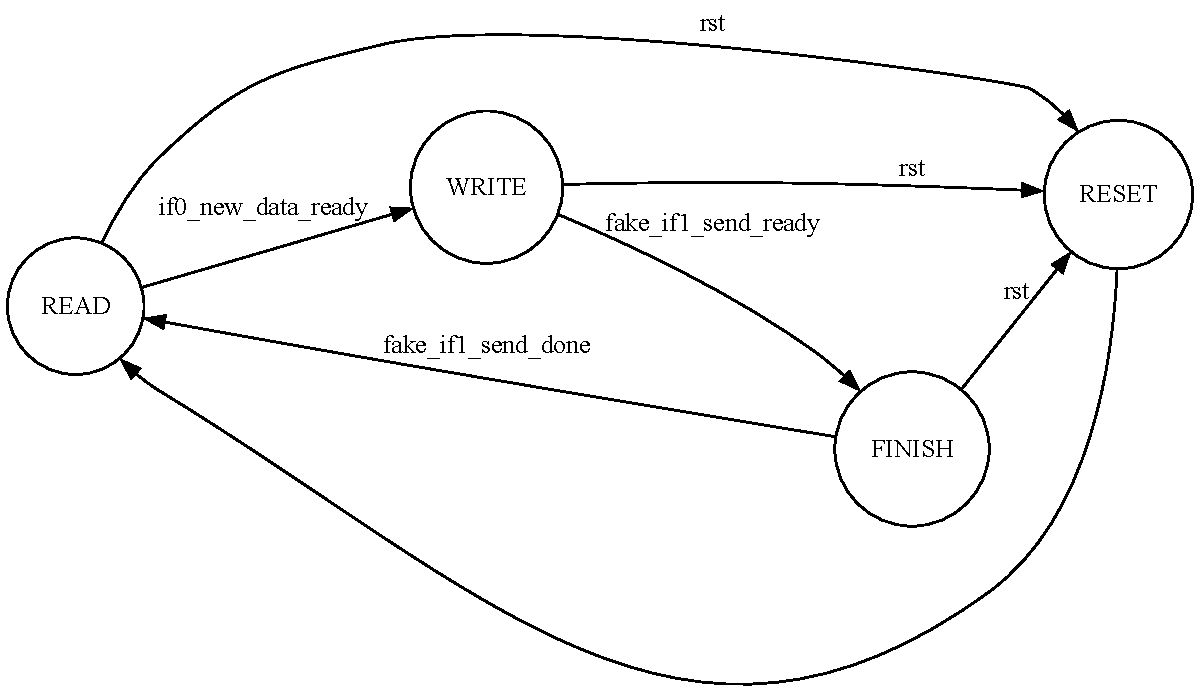
\includegraphics[width=1\textwidth]{images/misc/mitmStateTransition.pdf}}
    \caption[Prechodový diagram stavov MITM logiky]{Prechodový diagram stavov MITM logiky. Znázornený diagram je pre smer komunikácie IF0->IF1. Logika prechodov pre opačný smer je analogická.}
    \label{obr:mitmStateTransition}
\end{figure}

V rámci MITM logiky definujeme okrem transparentného režimu, tri ukážkové falošné režimy. V prvom režime nahrádzame v jednom smere ľubovoľnú hodnotu za konštantu 0x23 (ASCI hodnota znaku \#) a v opačnom smere komunikáciu úplne blokujeme. (V stave \texttt{WRITE} nezapneme signál pre spustenie vysielania.) Ďalší falošný režim bude symetrický, pričom vymeníme smer, v ktorom nahrádzame dáta konštantou, so smerom, v ktorom komunikáciu blokujeme. Ako konštantu budeme tentokrát posielať hodnotu 0x24 (ASCI hodnota znaku \$). V poslednom režime budeme nad vybranými dátami realizovať transformáciu ROT13 oboma smermi. Pokiaľ prečítame hodnotu z rozsahu A--Z alebo a--z, dáta zrotujeme, v opačnom prípade pošleme hodnotu, ktorú sme prečítali.

\subsection{Konfigurácia a syntéza FPGA obvodu}
Ďalej je potrebné nakonfigurovať parametre v súbore \texttt{config.vh}. Najdôležitejším parametrom je frekvencia systémových hodín, ktorého obmedzenia sme spomenuli v časti \ref{subsek:sysFreq}. Pre tento účel je najskôr potrebné určiť symbolovú rýchlosť zbernice UART. V našom prípade budeme používať štandardnú rýchlosť 115\,200, čo v zodpovedá 115.2\,kHz. Táto frekvencia vysielania dát je približná nakoľko UART protokol povoľuje odchýlku 5\%. Frekvenciu systémových hodín nastavíme preto na 16\,MHz, čo je minimálna hodnota, ktorú je použitý PLL obvod schopný generovať. Ďalšie parametre, ktoré je potrebné upraviť sú spomenutá symbolová rýchlosť, počet bitov jedného rámca -- v prípade štandardnej UART komunikácie 8 a počet režimov MITM logiky, ktoré sme v predošlej časti \ref{subsek:uartMitmLogic} definovali štyri. Parametre týkajúce sa SPI zbernice nemusíme konfigurovať. Ostatné parametre ponecháme na predvolenej hodnote. V tabuľke \ref{tab:uartConfig} nakonfigurované hodnoty všetkých relevantných parametrov.

\begin{table}
    \caption[Príklad konfigurácie parametrov pre UART]{Príklad konfigurácie parametrov pre UART.}
    \label{tab:uartConfig}
    \begin{center}
    \begin{tabular}{V{4}c|cV{4}}
        \hlineB{4}
        Parameter & Hodnota \\
        \hlineB{4}
        SYS\_FREQ & 16 \\
        \hline
        DEBOUNCE\_LEN\_US & 50\,000 (predvolené nastavenie) \\
        \hline
        NUM\_MITM\_MODES & 4 \\
        \hline
        NUM\_DATA\_BITS & v8 \\
        \hline
        UART\_BAUD\_RATE & 115\,200 \\
        \hlineB{4}
    \end{tabular}
    \end{center}
\end{table}

V tomto príklade budeme syntetizovať obvod pre dosku icestick. Fyzické mapovanie vstupov a výstupov ponecháme také ako je predvolené. Toto mapovanie bude dôležité pri fyzickom zapojení FPGA obvodu v ďalšej časti. Následne môžeme spustiť syntézu FPGA obvodu príkazom \texttt{make icestick-uart}. Skript po úspešnej syntéze vygeneruje v adresári \texttt{build/bin/} binárny súbor s názvom \texttt{icestick-uart.bin}, ktorý možno nahrať na FPGA dosku pomocou programu iceprog. Postup pri nahraní konfigurácie na FPGA závisí od použitého operačného systému a nainštalovaného ovládača pre FPGA dosku.

\subsection{Fyzické zapojenie hardvéru}
Po nahraní konfigurácie na FPGA je potrebné správne zapojiť hardvérové komponenty k FPGA doske -- jednotlivé vodiče použitej zbernice (v našom prípade UART) a tlačidlá pre globálny reset a zmenu MITM režimu. Výstupné LED diódy sa nachádzajú priamo na doske, v prípade potreby je však možné upraviť mapovanie fyzických výstupov a pripojiť vlastné LED diódy k zvoleným výstupom.

Pre demonštráciu funkčnosti implementovanej MITM logiky použijeme dva prevodníky z USB na UART, ktoré pripojíme k počítaču a budeme simulovať komunikáciu pomocou sériového terminálu. Nižšie uvádzame kompletný zoznam použitého hardvéru:
\begin{itemize}
    \item FPGA vývojová doska iCEstick Evaluation Kit
    \item dva prevodníky medzi USB a UART s čipom CP2102
    \item kontaktné bez-spájkové pole
    \item dve spínacie tlačidlá
    \item prepojovacie kábliky
\end{itemize}
Hardvér zapojíme podľa schémy na obrázku \ref{obr:schemeUartMitm}.

\begin{figure}
    \centerline{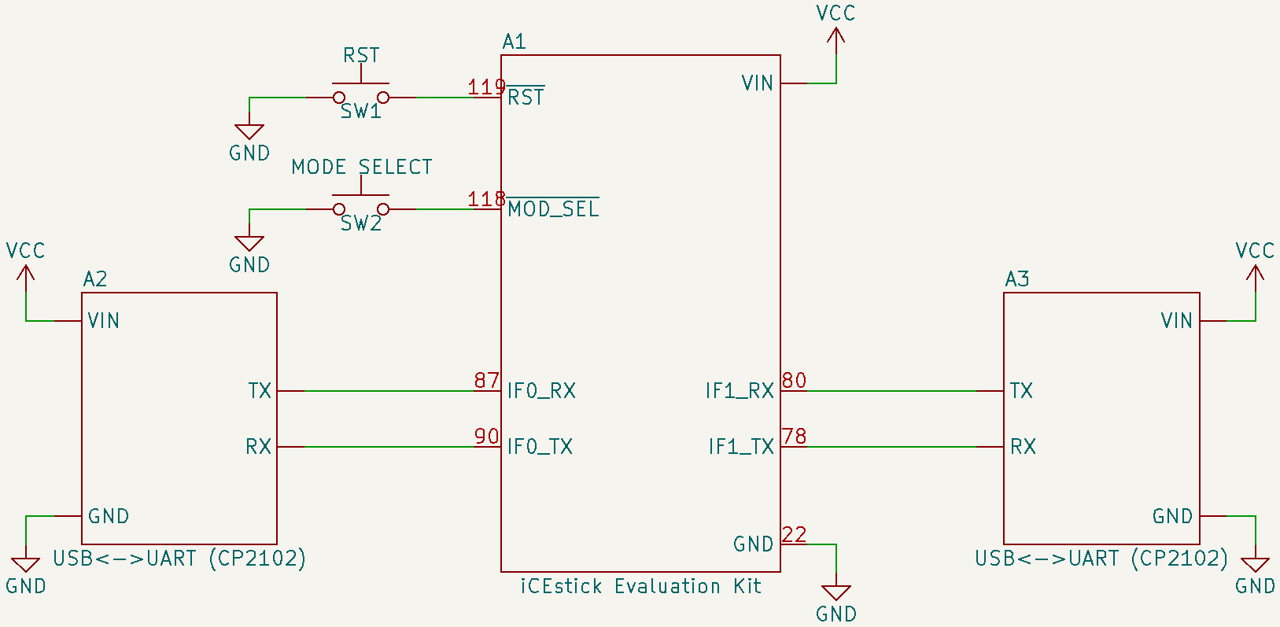
\includegraphics[width=1\textwidth]{images/schematics/schemeUartMitm.png}}
    \caption[Schéma zapojenia FPGA MITM obvodu pre UART]{Schéma zapojenia FPGA MITM obvodu pre UART.}
    \label{obr:schemeUartMitm}
\end{figure}

Funkcionalitu môžeme následne demonštrovať na jednoduchom scenári: USB konce prevodníkov pripojíme k všeobecnému počítaču. Zároveň zapojíme cez USB aj samotnú dosku icestick kvôli napájaniu (Dátová komunikácia medzi PC a doskou icestick už nie je potrebná, nakoľko FPGA konfiguráciu sme na dosku nahrali v predošlom kroku.) Následne môžeme otvoriť dva virtuálne sériové terminály pripojené k USB prevodníkom. V transparentnom režime MITM logiky sa všetok vstup do prvého terminálu zobrazí na druhom (a naopak). Prepínaním medzi režimami MITM logiky pomocou príslušného tlačidla možno vidieť realizáciu zásahov do komunikácie pri rôznych režimoch, ktoré sme opísali v časti \ref{subsek:uartMitmLogic}.

\section{Príklad 2 -- útok na komunikáciu s TPM} \label{sek:example2}
V tejto časti predstavíme o niečo komplexnejší útok na komunikáciu medzi mikrokontrolérom a externým TPM modulom. Na mikrokontroléri implementujeme program, ktorý bude periodicky získavať pomocou náhodne generované čísla pomocou TPM. Následne medzi TPM a mikrokontrolér zapojíme náš FPGA obvod, na ktorom implementujeme MITM logiku, ktorá bude modifikovať náhodne vygenerované bity, napríklad za konštantné. Konkrétne použijeme mikrokontrolér ESP8266, ktorý bude cez FPGA pripojený k TPM modulu SLB9670.

\subsection{TPM SPI protokol}
TPM štandard presne definuje spôsob komunikácie s TPM v prípade, že je použitá zbernica SPI \cite{tpmTis}. V tejto časti uvedieme niektoré detaily zo štandardu, relevantné pre porozumenie princípu útoku na generovanie náhodných čísel. TPM je v role slave zariadenia a komunikáciu riadi druhá strana. Počas SPI komunikácie je počet prenesených bitov (a teda hodinových taktov na SCLK linke) je vždy zarovnaný na celý bajtov. Bity v rámci bajtu sú vždy prenášané od najvýznamnejšieho bitu a rovnako v prípade viac-bajtových hodnôt sú bajty prenášané od najvýznamnejšieho. Štandard zároveň požaduje podporu pre SCLK mód 0 na TPM zariadení.

Na vyššej úrovni komunikácia s TPM prebieha čítaním a zápisom do špecifických TPM registrov. Čítanie a zápis do registra potom vyzerá nasledovne: Najvýznamnejší bit prvého bajtu (posielaný mastrom na MOSI linke) určuje či ide o operáciu čítania (1) alebo zápisu (0). Nasledovných sedem bitov predstavuje počet bajtov, ktoré chceme zapísať/prečítať mínus jeden. Napríklad 0x80 znamená, že chceme prečítať jeden bajt. Nasledujú tri bajty, ktoré určujú adresu registra. V prípade, že ide o operáciu zápisu po adrese nasledujú jednotlivé dáta, ktoré sa do registra majú uložiť. V prípade operácie čítania je potrebné ďalej taktovať na SCLK linke dostatočný počet bajtov, aby malo TPM priestor odpovedať. V princípe to znamená \uv{poslať} príslušný počet bajtov, na ktorých hodnote nezáleží a podstatné sú iba dáta vysielané z TPM po MISO linke. Na obrázku \ref{obr:tpmRW} je znázornené čítanie a zápis do TPM registra.

\begin{figure}
    \centering
    \subfloat[Prečítanie jedného bajtu (0x90) z registra 0xD40018.]{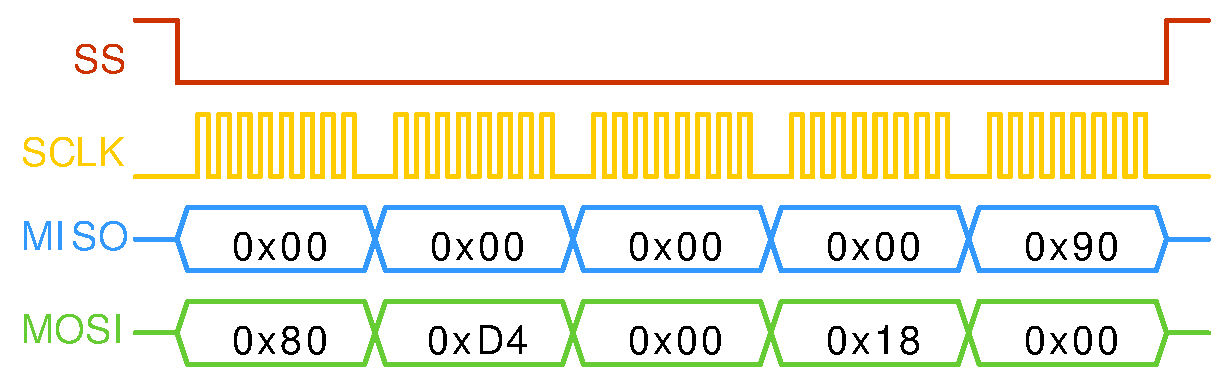
\includegraphics[width=1\textwidth]{images/signals/tpmRead.pdf}}
    \vfill
    \subfloat[Zápis dvoch bajtov (0x8001) do registra 0xD40024.]{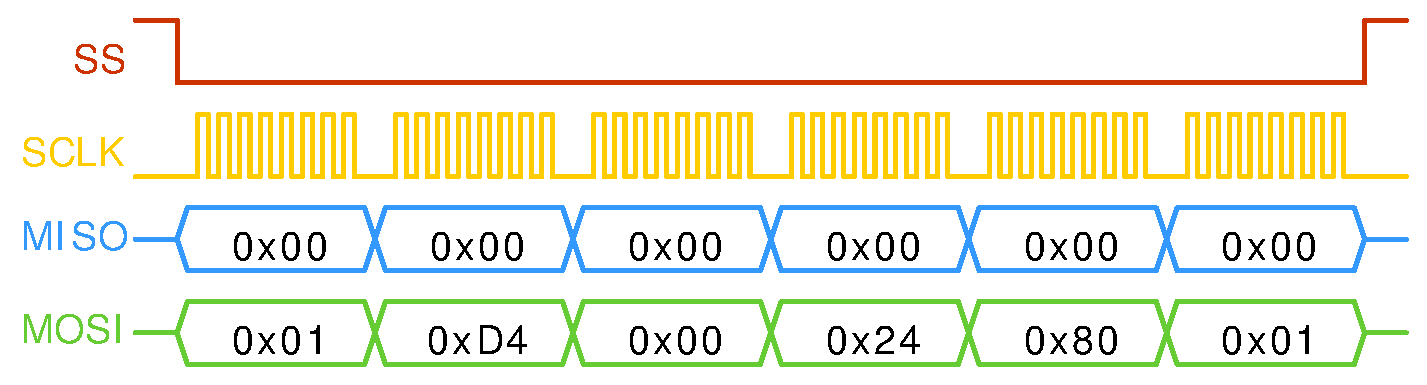
\includegraphics[width=1\textwidth]{images/signals/tpmWrite.pdf}}
    \caption[Komunikácia s TPM]{Komunikácia s TPM.}
    \label{obr:tpmRW}
\end{figure}

Jednotlivé registre sú adresované tzv. ofsetom od bázovej adresy. Bázová adresa sa na platformách zvykne využívať na zabezpečenie správneho mapovania TPM registrov do pamäte v prípade použitia memory mapped I/O. V našom jednoduchom prípade na bázovej adrese nezáleží, podstatné je aby počas celej komunikácie bola konštantná. Pre účely tejto práce spomenieme dva podstatné registre.

\textbf{TPM STATUS} register

\textbf{TPM FIFO} register

\subsection{MITM logika pre útok na komunikáciu s TPM}

\subsection{Fyzická realizácia útoku}